\chapter{Serialisation abstractions}
\label{serialisation}

Some of the various pieces of data that are handled by consensus also need to be
serialised to a binary format so that they can be:

\begin{enumerate}
\item written/read to/from \emph{storage} (see \cref{storage}) or;
\item sent/received across the \emph{network} (e.g., headers via the chain sync
  protocol \cref{chainsyncclient}).
\end{enumerate}

The two serialisation purposes above have different requirements and are
independent of each other. For example, when establishing a network connection,
a version number is negotiated. We can vary the network serialisation format
depending on the version number, allowing for instance to include some more
information in the payload. A concrete example of this is that starting from a
certain version, we include the block size in the payload when sending a
Byron\todo{Can I talk about Byron here?} header across the network as the header
itself does not contain it. This kind of versioning only concerns the network
and is independent of the storage layer. Hence we define separate abstractions
for them, decoupling them from each other.

For both abstractions, we use the CBOR (Concise Binary Object
Representation)\todo{command for acronyms?} format, because it has the following
benefits, paraphrasing the \texttt{cborg} library\todo{link?}:
\begin{itemize}
\item fast serialisation and deserialisation
\item compact binary format
\item stable format across platforms (32/64bit, big/little endian)
\item potential to read the serialised format from other languages
\item incremental or streaming (de)serialisation
\item suitable to use with untrusted input (resistance to asymmetric resource consumption attacks)
\item ...
\end{itemize}
Moreover, CBOR was chosen for the initial implementation of the Cardano
blockchain,\todo{correct?} with which we must maintain binary compatibility.
While it was possible to switch to another format for the block types developed
after the initial implementation, we saw no reason to switch.

We will now discuss both serialisation abstractions in more detail.

\section{Serialising for storage}
\label{serialisation:storage}

The following data is stored on disk (see \cref{storage}):

\begin{itemize}
\item Blocks
\item The extended ledger state (see \cref{storage:extledgerstate} and
  \cref{ledgerdb:on-disk}) which is the combination of:
  \begin{itemize}
  \item The header state (\cref{storage:headerstate})
  \item The ledger state\todo{link?}
  \end{itemize}
\end{itemize}

We use the following abstraction for serialising data to and from disk:

\begin{lstlisting}
class EncodeDisk blk a where
  encodeDisk :: CodecConfig blk -> a -> Encoding

class DecodeDisk blk a where
  decodeDisk :: CodecConfig blk -> forall s. Decoder s a
\end{lstlisting}

\begin{itemize}
\item These type classes have two type parameters: the block \lstinline!blk!,
  over which most things are parameterised, and \lstinline!a!, the type to
  (de)serialise. For example, \lstinline!a! can be the block type itself or the
  type corresponding to the ledger state.
\item \lstinline!CodecConfig blk! is a data family that defines the extra
  configuration needed for (de)serialisation. For example, to deserialise an EBB
  (\cref{ebbs}), the number of slots per epoch needs to be known statically to
  compute the slot of the block based on the epoch number, as the serialisation
  of an EBB does not contain its slot number, but the in-memory representation
  does. This configuration is kept as small as possible and is ideally empty.
\item The \lstinline!a -> Encoding! and \lstinline!forall s. Decoder s a! are
  the types for respectively encoders and decoders of the \lstinline!cborg!
  library.\todo{link?}
\item The encoder and decoder are split in two classes because they are not
  always \emph{symmetric}: the instantiation of \lstinline!a! in the encoder is
  not always the same as in the corresponding decoder. This is because blocks
  are \emph{annotated} with their serialisation. We discuss this in more detail
  in \cref{serialisation:annotations}.
\end{itemize}

\subsection{Nested contents}
\label{serialisation:storage:nested-contents}

By writing a block to disk we automatically have written the block's header to
disk, as the header is a part of the block. While we never write just a header,
we do support \emph{reading} just the header. This is more efficient than
reading the entire block and then extracting the header, as fewer bytes have to
be read from disk and deserialised.

\begin{center}
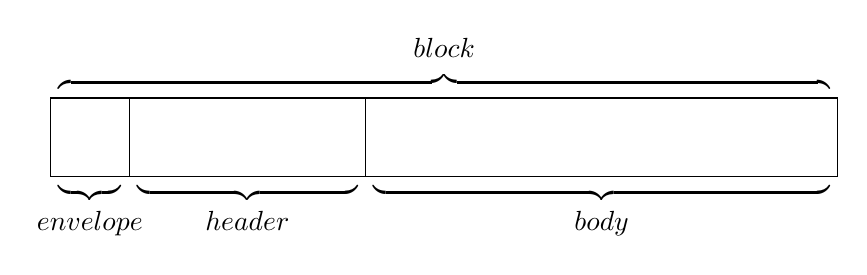
\begin{tikzpicture}
\draw  (0,    0)  -- (10,  0);
\draw  (0,    1)  -- (10,  1);
\draw  (0,    0)  --  (0,  1);
\draw  (1,    0)  --  (1,  1);
\draw  (4,    0)  --  (4,  1);
\draw (10,    0)  -- (10,  1);
\draw  (5,    1.2) node {$\overbrace{\hspace{9.8cm}}$};
\draw  (5,    1.6) node[fill=white] {$\mathstrut block$};
\draw  (0.5, -0.2) node {$\underbrace{\hspace{0.8cm}}$};
\draw  (0.5, -0.6) node[fill=white] {$\mathstrut envelope$};
\draw  (2.5, -0.2) node {$\underbrace{\hspace{2.8cm}}$};
\draw  (2.5, -0.6) node[fill=white] {$\mathstrut header$};
\draw  (7,   -0.2) node {$\underbrace{\hspace{5.8cm}}$};
\draw  (7,   -0.6) node[fill=white] {$\mathstrut body$};
\end{tikzpicture}
\end{center}

Extracting the header from a block on disk can be very simple, like in the
figure above. The block starts with an envelope, which is followed by the block
header and the block body. In this case, we read the bytes starting from the
start of the header until the end of the header, which we then decode. We use
the following abstraction to represent this information:

\begin{lstlisting}
data BinaryBlockInfo = BinaryBlockInfo {
      headerOffset :: !Word16
    , headerSize   :: !Word16
    }

class HasBinaryBlockInfo blk where
  getBinaryBlockInfo :: blk -> BinaryBlockInfo
\end{lstlisting}

As the size of a header can vary on a per-block basis, we maintain this
information \emph{per block} in the storage layer.\todo{link?} We trade four
extra bytes of storage and memory space for faster reading of headers.

However, it is not for every type of block the case that the encoding of a
header can literally be sliced out of the encoding of the corresponding block.
The serialisation of a header when embedded in a block might be different from
the serialisation of a header on its own. For example, the standalone header
might require an additional envelope or a different one than the block's
envelope.

A concrete example of this are the Byron blocks and headers. A Byron block is
either a regular block or an epoch boundary block (EBB) (discussed in
\cref{ebbs}). A regular block has a different header than an EBB, consequently,
their encoding differs. The envelope of the encoding of a Byron block includes a
tag indicating whether the block is a regular block or an EBB, so that the
decoder knows what kind of header and body to expect. For the same reason, the
envelope of the encoding of a standalone Byron header includes the same tag.
However, when we slice out the header from the Byron block and feed that to the
decoder for Byron headers, the envelope containing the tag will be
\emph{missing}.

The same problem presents itself for the hard fork combinator (\cref{hfc}): when
using the hard fork combinator to combine two block types, A and B, into one,
the block's envelope will (typically) indicate whether it is a block of type A
or B. The header corresponding to such a block will have a similar envelope.
When we slice the header out of such a block, the required envelope will be
missing. The right envelope has to be prepended so that the header decoder knows
whether it should expect A or B.

The header is \emph{nested} inside the block and to be able to decode it, we
need some more \emph{context}, i.e., the envelope of the header. In the storage
layer (\cref{storage}), we store the context of each block in an index
(in-memory or on-disk, depending on the database) so that after reading both the
context and the sliced header, we can decode the header without having to read
and decode the entire block. We capture this idea in the following abstractions.

\begin{lstlisting}
data family NestedCtxt_ blk :: (Type -> Type) -> (Type -> Type)
\end{lstlisting}
As usual, we parameterise over the block type. We also parameterise over another
functor, e.g., \lstinline!f!, which in practice will be instantiated to
\lstinline!Header!, but in the future, there might be more types of nested
contents, other than headers, e.g., block bodies. The constructors of this data
family will represent the different types of context available, e.g., for Byron
a context for regular blocks and a context for EBBs.

\lstinline!NestedCtxt! is indexed by \lstinline!blk!: it is the block that
determines this type. However, we often want to partially apply the second
argument (the functor), leaving the block type not yet defined, hence we define:
\begin{lstlisting}
newtype NestedCtxt f blk a = NestedCtxt {
      flipNestedCtxt :: NestedCtxt_ blk f a
    }
\end{lstlisting}
The \lstinline!a! type index will correspond to the raw, sliced header that
requires the additional context. It can vary with the context, e.g., the context
for a Byron EBB will fix \lstinline!a! to a raw EBB header (without the
necessary envelope).

Now that we have defined \lstinline!NestedCtxt!, we can define the class that
allows us to separate the nested type (the header) into the context and the raw,
sliced type (the raw header, \lstinline!a!), as well as the inverse:
\begin{lstlisting}
class (..) => HasNestedContent f blk where
  unnest :: f blk -> DepPair (NestedCtxt f blk)
  nest   :: DepPair (NestedCtxt f blk) -> f blk
\end{lstlisting}
\lstinline!DepPair! is a dependent pair that allows us to hide the type
parameter \lstinline!a!. When writing a block, \lstinline!unnest! is used to
extract the context so that it can be stored in the appropriate index. When
reading a header, \lstinline!nest! is used to combine the context, read from the
appropriate index, with the raw header into the header.

In certain scenarios, we do not have access to the separately stored context of
the block, but we do have access to the encoded block, in which case we should
be able to able to extract the context directly from the encoded block, without
having to decode it entirely. We use the \lstinline!ReconstructNestedCtxt! class
for this:
\begin{lstlisting}
class HasNestedContent f blk => ReconstructNestedCtxt f blk where
  reconstructPrefixLen  :: proxy (f blk) -> PrefixLen
  reconstructNestedCtxt ::
       proxy (f blk)
    -> ShortByteString
    -> ..
    -> SomeSecond (NestedCtxt f) blk
\end{lstlisting}
The \lstinline!PrefixLen! is the number of bytes extracted from the beginning of
the encoded block required to reconstruct the context. The
\lstinline!ShortByteString! corresponds to these bytes. The
\lstinline!reconstructNestedCtxt! method will parse this bytestring and return
the corresponding context. The \lstinline!SomeSecond! type is used to hide the
type parameter \lstinline!a!.

As these contexts and context-dependent types do not fit the mould of the
\lstinline!EncodeDisk! and \lstinline!DecodeDisk! classes described in
\cref{serialisation:storage}, we define variants of these classes:
\begin{lstlisting}
class EncodeDiskDepIx f blk where
  encodeDiskDepIx :: CodecConfig blk
                  -> SomeSecond f blk -> Encoding

class DecodeDiskDepIx f blk where
  decodeDiskDepIx :: CodecConfig blk
                  -> Decoder s (SomeSecond f blk)

class EncodeDiskDep f blk where
  encodeDiskDep :: CodecConfig blk -> f blk a
                -> a -> Encoding

class DecodeDiskDep f blk where
  decodeDiskDep :: CodecConfig blk -> f blk a
                -> forall s. Decoder s (ByteString -> a)
\end{lstlisting}
\todo{explain?}

\section{Serialising for network transmission}
\label{serialisation:network}

The following data is sent across the network:
\begin{itemize}
\item Header hashes
\item Blocks
\item Headers
\item Transactions
\item Transaction IDs
\item Transaction validation errors
\item Ledger queries
\item Ledger query results
\end{itemize}
\todo{less whitespace}

We use the following abstraction for serialising data to and from the network:

\begin{lstlisting}
class SerialiseNodeToNode blk a where
  encodeNodeToNode :: CodecConfig blk
                   -> BlockNodeToNodeVersion blk
                   -> a -> Encoding
  decodeNodeToNode :: CodecConfig blk
                   -> BlockNodeToNodeVersion blk
                   -> forall s. Decoder s a

class SerialiseNodeToClient blk a where
  encodeNodeToClient :: CodecConfig blk
                     -> BlockNodeToClientVersion blk
                     -> a -> Encoding
  decodeNodeToClient :: CodecConfig blk
                     -> BlockNodeToClientVersion blk
                     -> forall s. Decoder s a
\end{lstlisting}

These classes are similar to the ones used for storage
(\cref{serialisation:storage}), but there are some important differences:

\begin{itemize}
\item The encoders and decoders are always symmetric, which means we do not have
  to separate encoders from decoders and can merge them in a single class.
  Nevertheless, some of the types sent across the network still have to deal
  with annotations (\cref{serialisation:annotations}), we discuss how we solve
  this in \cref{serialisation:network:cbor-in-cbor}.
\item We have separate classes for \emph{node-to-node} and \emph{node-to-client}
  serialisation.\todo{link?}
  By separating them, we are more explicit about which data is serialised for
  which type of connection. Node-to-node protocols and node-to-client protocols
  have different properties and requirements. This also gives us the ability to,
  for example, use a different encoding for blocks for node-to-node protocols
  than for node-to-client protocols.
\item The methods in these classes all take a \emph{version} as argument. We
  will discuss versioning in \cref{serialisation:network:versioning}.
\end{itemize}

\subsection{Versioning}
\label{serialisation:network:versioning}

As requirements evolve, features are added, data types change, constructors are
added and removed. For example, adding the block size to the Byron headers,
adding new ledger query constructors, etc. This affects the data we send across
the network. In a distributed network of nodes, it is a given that not all nodes
will simultaneously upgrade to the latest released version and that nodes
running different versions of the software, i.e., different versions of the
consensus layer, will try to communicate with each other. They should of course
be able to communicate with each other, otherwise the different versions would
cause partitions in the network.

This means we should be careful to maintain binary compatibility between
versions. The network layer is faced with the same issue: as requirements
evolve, network protocols (block fetch, chain sync\todo{link?}) are modified
change (adding messages, removing messages, etc.), network protocols are added
or retired, etc. While the network layer is responsible for the network
protocols and the encoding of their messages, the consensus layer is responsible
for the encoding of the data embedded in these messages. Changes to either
should be possible without losing compatibility: a node should be able to
communicate successfully with other nodes that run a newer or older version of
the software, up to certain limits (old versions can be retired eventually).

To accomplish this, the network layer uses \emph{versions}, one for each bundle
of protocols:
\begin{lstlisting}
data NodeToNodeVersion
    = NodeToNodeV_1
    | NodeToNodeV_2
    | ..

data NodeToClientVersion
    = NodeToClientV_1
    | NodeToClientV_2
    | ..
\end{lstlisting}
For each backwards-incompatible change, either a change in the network protocols
or in the encoding of the consensus data types, a new version number is
introduced in the corresponding version data type. When the network layer
establishes a connection with another node or client, it will negotiate a
version number during the handshake: the highest version that both parties can
agree on. This version number is then passed to any client and server handlers,
which decide based on the version number which protocols to start and which
protocol messages (not) to send. A new protocol message would only be sent when
the version number is greater or equal than the one with which it was
introduced.

This same network version is passed to the consensus layer, so we can follow the
same approach. However, we decouple the network version numbers from the
consensus version numbers for the following reason. A new network version number
is needed for each backwards-incompatible change to the network protocols or the
encoding of the consensus data types. This is clearly a strict superset of the
changes caused by consensus. When the network layer introduces a new protocol
message, this does not necessarily mean anything changes in the encoding of the
consensus data types. This means multiple network versions can correspond to the
same consensus-side encoding or \emph{consensus version}. In the other
direction, each change to the consensus-side encodings should result in a new
network version. We capture this in the following abstraction:
\begin{lstlisting}
class (..) => HasNetworkProtocolVersion blk where
  type BlockNodeToNodeVersion   blk :: Type
  type BlockNodeToClientVersion blk :: Type

class HasNetworkProtocolVersion blk
   => SupportedNetworkProtocolVersion blk where
  supportedNodeToNodeVersions ::
       Proxy blk -> Map NodeToNodeVersion   (BlockNodeToNodeVersion   blk)
  supportedNodeToClientVersions ::
       Proxy blk -> Map NodeToClientVersion (BlockNodeToClientVersion blk)
\end{lstlisting}
The \lstinline!HasNetworkProtocolVersion! class has two associated types to
define the consensus version number types for the given block. When no
versioning is needed, one can use the unit type as the version number. The
\lstinline!SupportedNetworkProtocolVersion! defines the mapping between the
network and the consensus version numbers. Note that this does not have to be an
injection, as multiple network version can most certainly map to the same
consensus version. Nor does this have to be a surjection, as old network and
consensus versions might be removed from the mapping when the old version no
longer needs to be supported. This last reason is also why this mapping is
modelled with a \lstinline!Map! instead of a function: it allows enumerating a
subset of all defined versions, which is not possible with a function.

\todo{TODO} Global numbering vs multiple block types

The \lstinline!SerialiseNodeToNode! and \lstinline!SerialiseNodeToClient!
instances can then branch on the passed version to introduce changes to the
encoding format, for example, the inclusion of the block size in the Byron
header encoding.

Consider the following scenario: a change is made to one of the consensus data
types, for example, a new query constructor is added the ledger query data type.
This requires a new consensus and thus network version number, as older versions
will not be able to decode it. What should be done when the new query
constructor is sent to a node that does not support it (the negotiated version
is older than the one in which the constructor was added)? If it is encoded and
send, the receiving side will fail to decode it and terminate its
connection.\todo{right?} This is rather confusing to the sender, as they are
left in the dark. Instead, we let the \emph{encoder} throw an exception in this
case, terminating that connection, so that the sender is at least notified of
this. \todo{TODO} Ideally, we could statically prevent such cases.

\subsection{CBOR-in-CBOR}
\label{serialisation:network:cbor-in-cbor}

In \cref{serialisation:annotations}, we explain why the result of the decoder
for types using \emph{annotations} needs to be passed the original encoding as a
bytestring. When reading from disk, we already have the entire bytestring in
memory,\todo{explain why} so it can easily be passed to the result of the
decoder. However, this is not the case when receiving a message via the network
layer: the entire message, containing the annotated type(s), is decoded
incrementally.\todo{right?} When decoding CBOR, it is not possible to obtain the
bytestring corresponding to what the decoder is decoding. To work around this,
we use \emph{CBOR-in-CBOR}: we encode the original data as CBOR and then encode
the resulting bytestring as CBOR \emph{again}. When decoding CBOR-in-CBOR, after
decoding the outer CBOR layer, we have exactly the bytestring that we will need
for the annotation. Next, we feed this bytestring to the original decoder, and,
finally, we pass the bytestring to the function returned by the decoder.

\subsection{Serialised}
\label{serialisation:network:serialised}

One of the duties of the consensus layer is to serve blocks and headers to other
nodes in the network.\todo{link?} To serve for example a block, we read it from
disk, deserialise it, and then serialise it again and send it across the
network. The costly deserialisation and serialisation steps cancel each other
out and are thus redundant. We perform this optimisation in the following way.
When reading such a block from storage, we do not read the \lstinline!blk!, but
the \lstinline!Serialised blk!, which is a phantom type around a raw, still
serialised bytestring:
\begin{lstlisting}
newtype Serialised a = Serialised ByteString
\end{lstlisting}
To send this serialised block over the network, we have to encode this
\lstinline!Serialised blk!. As it happens, we use CBOR-in-CBOR to send both
blocks and headers over the network, as described in
\cref{serialisation:network:cbor-in-cbor}. This means the serialised block
corresponds to the inner CBOR layer and that we only have to encode the
bytestring again as CBOR, which is cheap.

This optimisation is only used to \emph{send} and thus encode blocks and
headers, not when \emph{receiving} them, because each received block or header
will have to be inspected and validated, and thus deserialised anyway.

As discussed in \cref{serialisation:storage:nested-contents}, reading a header
(nested in a block) from disk requires reading the context and the raw header,
and then combining them before we can deserialise the header. This means the
approach for serialised headers differs slightly:
\begin{lstlisting}
newtype SerialisedHeader blk = SerialisedHeaderFromDepPair {
      serialisedHeaderToDepPair :: GenDepPair Serialised
                                              (NestedCtxt Header blk)
    }
\end{lstlisting}
This is similar to the \lstinline!DepPair (NestedCtxt f blk)! type from
\cref{serialisation:storage:nested-contents}, but this time the raw header is
wrapped in \lstinline!Serialised! instead of being deserialised.

\section{Annotations}
\label{serialisation:annotations}

\todo{TODO} move up? The previous two sections refer to this

The following technique is used in the Byron and Shelley ledgers for a number of
data types like blocks, headers, transactions, \ldots The in-memory representation
of, for example a block, consists of both the typical fields describing the
block (header, transactions, \ldots), but also the \emph{serialisation} of the block
in question. The block is \emph{annotated} with its serialisation.

The principal reason for this is that it is possible that multiple
serialisations, each which a different hash, correspond to the same logical
block. For example, a client sending us the block might encode a number using a
binary type that is wider than necessary (e.g., encoding the number 0 using four
bytes instead of a single byte). CBOR defines a \emph{canonical format}, we call
an encoding that is in CBOR's canonical format a \emph{canonical
encoding}.\todo{link?}

When after deserialising a block in a non-canonical encoding, we serialise it
again, we will end up with a different encoding, i.e., the canonical encoding,
as we stick to the canonical format. This means the hash, which is part of the
blockchain, is now different and can no longer be verified.

For this reason, when deserialising a block, the original, possibly
non-canonical encoding is retained and used to annotate the block. To compute
the hash of the block, one can hash the annotated serialisation.

Besides solving the issue with non-canonical encodings, this has a performance
advantage, as encoding such a block is very cheap, it is just a matter of
copying the in-memory annotation.

\todo{TODO} We rely on it being cheap in a few places, mention that/them?

\todo{TODO} extra memory usage

This means that the result of the decoder must be passed the original encoding
as a bytestring to use as the annotation of the block or other type in question.
Hence the decoder corresponding to the encoder \lstinline!blk -> Encoding! has
type \lstinline!forall s. Decoder s (ByteString -> blk)!, which is a different
instantiation of the type \lstinline!a!, explaining the split of the
serialisation classes used for storage (\cref{serialisation:storage}). The
original encoding is then applied to the resulting function to obtain the
annotated block. This asymmetry is handled in a different way for the network
serialisation, namely using CBOR-in-CBOR
(\cref{serialisation:network:cbor-in-cbor}).

\subsection{Slicing}

\todo{TODO} discuss the slicing of annotations with an example. What is the
relation between the decoded bytestring and the bytestring passed to the
function the decoder returns? Talk about compositionality.
